\chapter{Implementación General}


\section{Simulación}

Antes de plantear un experimento real decidimos probar nuestro sistema en un caso experimental, para eso se decidió usar \textit{NS3}. \textit{NS3} es un simulador de redes que permite no solo emular protocolos de enrutamiento como \textbf{AODV} (\textit{Ad hoc On-Demand Distance Vector Routing}) sino también aplicarle movilidad a los nodos y utilizar distintos modelos de \textit{Path Loss}.

Para este experimento simulado se decidió configurar una red \textit{Ad Hoc} entre todos los nodos. Y se usó un modelo de propagación ideal, el \textbf{ns3::FriisPropagationLossModel}.
Uno de los nodos, nuestro \textbf{Objetivo}, se configuró como el nodo transmisor. Este emite mensajes constantemente de tipo \textit{broadcast} que al estar conectados en una red \textit{ad hoc} todos reciben.
Cada nodo tiene un script que al recibir un mensaje de \textit{broadcast} del nodo \textbf{Objetivo} guarda la ubicación real de este y el \textbf{RSSI} con el que se recibió el paquete.
Mientras esto ocurre, usando un modelo de movilidad, se le aplica un recorrido al nodo \textbf{objetivo}. Mientras tanto a los otros nodos, que hacen las veces de \textit{Sniffer}, permanecen quietos durante todo el experimento. Al finalizar la simulación se recopilan los datos en un archivo \textit{.csv} para luego ser analizados por herramientas propias.

\subsection{Perfilado}

\begin{figure}[!htb]
	\centering
\includegraphics[width=0.5\textwidth]{Figuras/profiling/simulation/profiling_pyvis_going_away2.jpg}
	\captionsetup{margin=2cm}
	\caption[Visualización de la simulacion de NS3. El nodo objetivo se aleja del nodo Sniffer.]{Visualización de la simulacion de NS3. El nodo objetivo se aleja de uno de los nodos Sniffer.}
	\label{fig:infra-diagram}
\end{figure}
 
En el caso del experimento de perfilado simulado, se utilizó un solo nodo \textit{Sniffer} que recibe paquetes de un nodo \textit{Objectivo} a medida que este se aleja. El resultado de la simulación es un archivo \textit{CSV} compuesto por filas (\textbf{distancia,rssi}). Finalmente tomamos estos datos de RSSI, mas los datos reales de distancia (calculados en la misma simulación) y realizamos un ajuste de curva hasta encontrar los valores de N Y A. Estos nos servirán mas adelante para predecir la distancia de dicho nodo en base a su RSSI.
 El código para este experimento se encuentra en el siguiente archivo \href{https://github.com/agusalex/ns3-rssi-trilateration/blob/main/src/1DDistanceProfiling.cc}{\textbf{1DDistanceProfiling.cc}}.
Finalmente se graficó la señal y la curva usando la librería \textit{pyplot}.


\subsection{Multilateracion}

Similar al experimento simulado de perfilado se utilizo \textbf{NS3}, esta vez con mas nodos y haciendo un recorrido en dos dimensiones. Se utilizo el siguiente archivo para ejecutar la simulación \href{https://github.com/agusalex/ns3-rssi-trilateration/blob/main/src/2DTrilateration.cc}{\textbf{2DTrilateration.cc}}. El resultado de la ejecución da otro archivo .csv con las siguientes columnas: \textbf{millis, x, y, rssi, target\_x, target\_y}. \textbf{Millis} representa los milisegundos de la simulación, esto se usara luego para agrupar por ese criterio a la hora de hacer la trilateración. \textbf{X} e \textbf{Y} representan la ubicación del nodo que capturo el \textbf{rssi} de esa medicion. Finalmente \textbf{target\_x} y \textbf{target\_y} son la ubicación real del nodo objetivo cuando la medición fue realizada, esto lo sabemos con certeza dado que el entorno es simulado.

\begin{table}[!htb]
\centering
\begin{tabular}{|c|c|c|c|c|c|c|c|}
\hline
millis & node & x & y & rssi & distance & target\_x & target\_y \\
\hline
9 & 2 & 12.5 & 0 & -63.5639 & 12.492 & 12.492 & 12.492 \\
9 & 4 & 25 & 12.5 & -63.5649 & 12.508 & 12.492 & 12.492 \\
9 & 5 & 0 & 12.5 & -63.5639 & 12.492 & 12.492 & 12.492 \\
9 & 7 & 12.5 & 25 & -63.5649 & 12.508 & 12.492 & 12.492 \\
9 & 1 & 0 & 0 & -68.0793 & 17.6664 & 12.492 & 12.492 \\
9 & 3 & 25 & 0 & -68.0799 & 17.6777 & 12.492 & 12.492 \\
9 & 6 & 0 & 25 & -68.0799 & 17.6777 & 12.492 & 12.492 \\
9 & 8 & 25 & 25 & -68.0804 & 17.689 & 12.492 & 12.492 \\
\hline
\end{tabular}
\caption{Captura simulada que luego se usara de input para multilateración. (Simulation.csv)}
\label{table:1}
\end{table}

Este archivo luego es procesado por nuestro algoritmo de multilateración, utilizando los valores de \textbf{A} y \textbf{N} hallados anteriormente para el perfilado simulado. Nuestro algoritmo de multilateración primero agrupa por paquetes que se hayan capturado al mismo momento, es decir que los milisegundos (\textbf{Millis}) de la simulación sean los mismos. Luego solo se le aplicara multilateración y de manera subsecuente se agregaran al recorrido aquellos grupos de paquetes que al menos hayan sido capturados por 4 nodos o mas. Esto se debe a que nuestro algoritmo de cuadrados mínimos necesita como mínimo al menos 4 nodos distintos para producir una predicción. Finalmente se graficó el recorrido en 2d usando al librería \textit{pyplot}.

\section{Experimento de campo preliminar de Perfilado Con \textbf{“\textit{steps}”} }
\begin{figure}[!htb]
	\centering
	\includegraphics[width=0.7\textwidth]{Figuras/infraestructure/arduino-rpi.png}
	\captionsetup{margin=2cm}
	\caption[Flujo de datos en mediciones de perfilado]{Flujo de datos en mediciones de perfilado. El Arduino transfiere los datos mientras llegan directamente a la RPI mediante USB. Estos se agrupan por distancia (ingresada por el usuario) gracias al al script de captura.}
	\label{fig:infra-diagram-arduino}
\end{figure}
\begin{figure}[!htb]
	\centering
	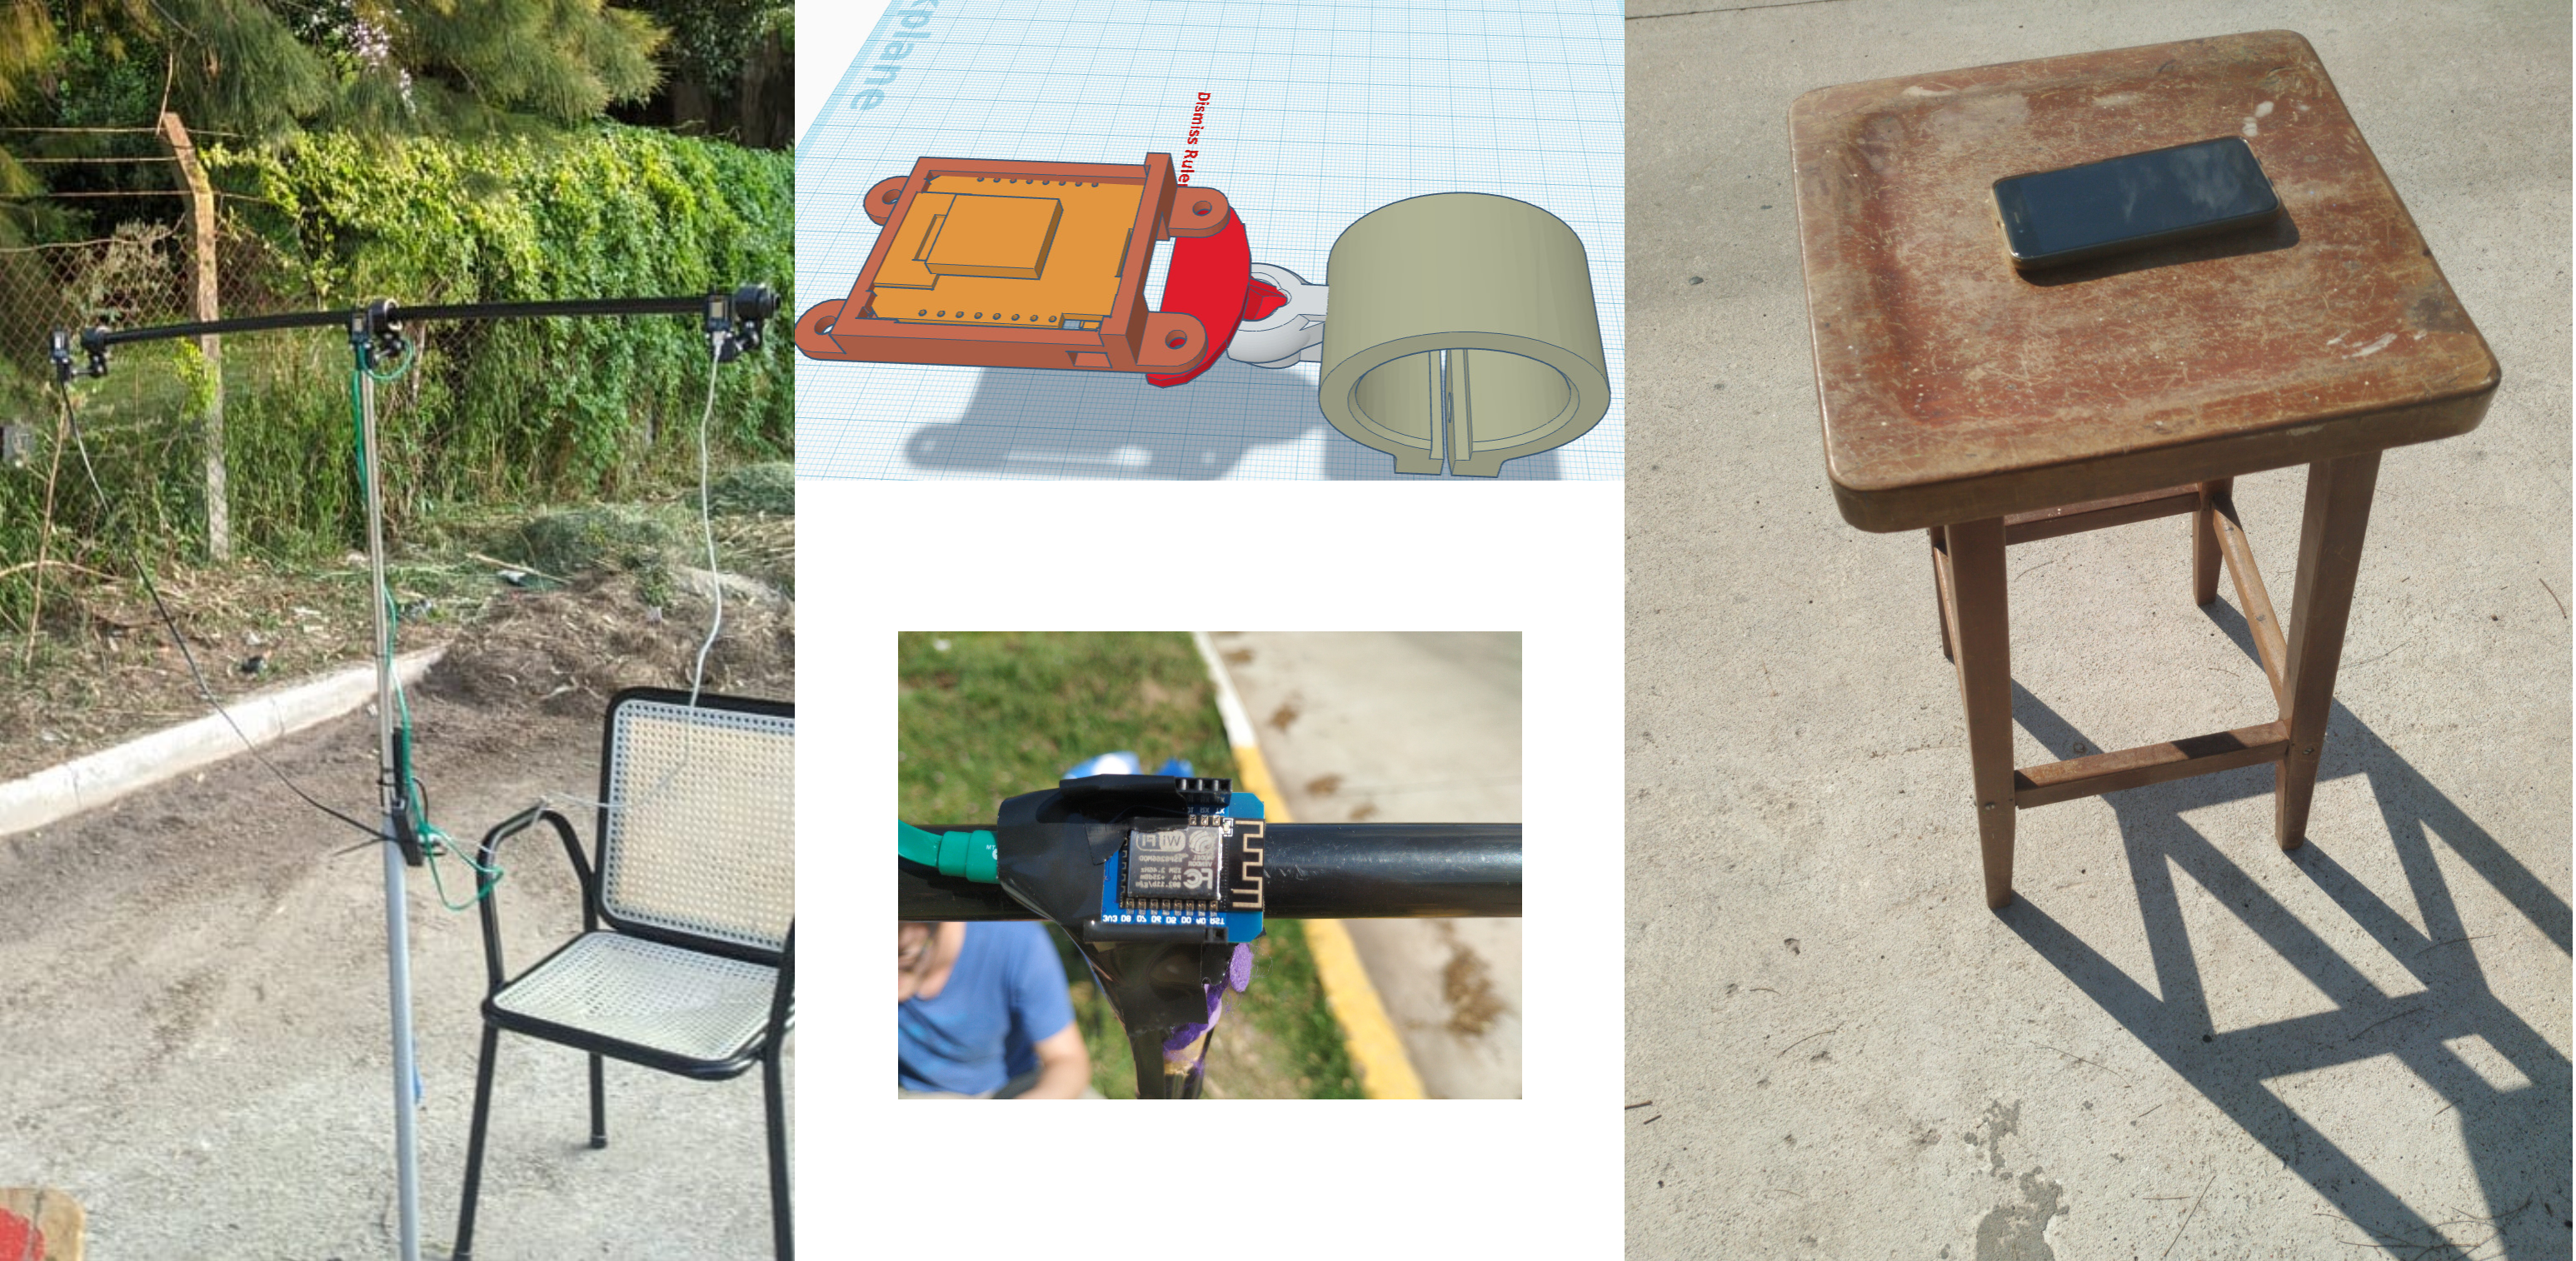
\includegraphics[width=0.8\textwidth]{Figuras/fieldwork/profiling-setup.png}
	\captionsetup{margin=2cm}
	\caption[Perfilado]{Experimento de campo de perfilado. Para que todos los dispositivos tengan sus antenas orientadas en el
mismo ángulo hacia la misma ubicación durante todo el experimento se utilizo
un soporte de metal con monturas hechas con impresora 3D.}
	\label{fig:arduino-profiling-setup}
\end{figure}
Si bien se eligió utilizar una infraestructura \textit{wireless}, se realizo un experimento preliminar conectando tres \textbf{ESP8266} mediante USB a la \textbf{RPI} para tomar múltiples muestras a una distancia conocida y poder poner un corte entre muestra y muestra a medida que las recibíamos. De esta manera poder etiquetar 200 muestras a 2 metros, a 5 a 10 etc.

Para ello, antes de avanzar con el proyecto hacia la etapa de multilateración, se quiso confirmar primero que la relación \textit{RSSI} a distancia que informaban los \textbf{ESP8266} se acercaba a la realidad (es decir que se aproxime a lo que debería ser el ideal, o el modelo de \textit{Path Loss} antes visto). De esta manera se decidió hacer un experimento de perfilado en un ambiente controlado (en el campo de deportes de la UNGS con muy poca interferencia en la banda 2.4GHZ). Además se garantizo la precisión de los datos mediante la toma de 200 muestras por cada\textbf{ “\textit{step}”} de medición y se tomo nota de la distancia al receptor en cada uno de ellos.

Para tomar dichas mediciones con precisión se conectaron tres \textbf{ESP8266} directamente a una \textbf{RPI} por \textbf{USB} y estos transmitían los datos por dicho medio constantemente. Para recibir esta información se desarrollo un \href{https://github.com/agusalex/PacketSnifferServer}{script} que toma \textbf{M} muestras y luego se detiene a esperar a que el usuario le indique la nueva distancia a que se realizara la próxima medición. De esta manera se obtiene \textbf{M} muestras agrupadas por la distancia, a esto le llamamos\textbf{ “\textit{step}”}.

Por cada dispositivo se tomaron 21 mediciones a 4.5 metros de distancia entre cada medición, conteniendo 200 muestras cada una. Dos de los dispositivos finalizaron el experimento y uno sufrió un desperfecto y dejó de recibir. Como transmisor se utilizo un dispositivo móvil (en modo \textit{Access Point}) sobre un banco de madera el cual se fue alejando 4.5 metros en cada medición. La distancia total fue recorrida fue de 100 metros.

Como último paso, calculamos la media por cada “\textit{step}” de distancia para filtrar las anomalías de los datos. Finalmente se ejecutó una regresión logarítmica usando cuadrados mínimos, el resultado nos da un \textbf{A} y un \textbf{N} que podría ser utilizado en el paso de multilateración.
\section{Experimento de campo}
\begin{figure}[!htb]
	\centering
	\includegraphics[width=0.8\textwidth]{Figuras/infraestructure/arduino-rpi-multi.png}
	\captionsetup{margin=2cm}
	\caption[Flujo de datos en mediciones de multilateración]{Flujo de datos en mediciones de multilateración. Los Arduinos recolectan los datos hasta agotar el espacio en memoria o llegar a un limite establecido. Finalmente descargan toda la información en una RPI de manera inalámbrica. }
	\label{fig:infra-diagram-arduino}
\end{figure}
\begin{figure}[!htb]
	\centering
	\includegraphics[width=0.8\textwidth]{Figuras/fieldwork/esp-poles-2.png}
	\captionsetup{margin=2cm}
	\caption[Postes Nodo Multilateración]{ Nodos \textit{Sniffer}. Se construyeron con PVC utilizaron una base de cemento. El ESP8266 fue adherido con velcro al tuvo junto con una bateria de \textit{LI-ION} }
	\label{fig:infra-diagram-arduino}
\end{figure}

Se plantearon distintas alternativas de \textit{hardware} para poder cubrir el área más grande posible al menor costo. Se pensó en la utilización de \textit{routers} comerciales como los \textbf{Ubiquiti} usando un \textit{software} de código abierto como \textbf{OpenWRT}, también la posibilidad de usar \textbf{Raspberry Pi} o similares e incluso microcontroladores con \textit{Wi-Fi} compatibles con \textbf{Arduino} como el \textbf{ESP8266} y el \textbf{ESP32}. 

Cualquiera de estas soluciones trae consigo un problema ineludible: Los adaptadores \textit{Wi-Fi} hasta donde hemos podido investigar no pueden operar en modo promiscuo y de algún otro modo en simultáneo. Se planteó la posibilidad de usar dispositivos que cuentan con dos adaptadores de \textit{Wi-Fi}, uno para capturar paquetes \textit{Probe Request} y otro para evacuarlos hacia una base de datos centralizada para que luego puedan ser analizados pero no se encontró ninguno de bajo costo y de uso masivo.

Por esto fue elegida la alternativa de utilizar un solo dispositivo \textbf{ESP8266} como \textit{Sniffer} y un \textbf{Raspberry Pi 3} en modo \textit{Access Point} (En otro canal) para recibir los datos. Para facilitar las mediciones utilizamos un tuvo de \textit{PVC} con una base de cemento. El \textbf{ESP8266} fue adherido con \textit{velcro} al tuvo y se le agrego una bateria de \textit{LI-ION} conectada a \textbf{VIN} y \textbf{GND} del dispositivo.


El \textbf{ESP8266} fue programado utilizando \textit{Arduino} y \textit{Platformio} para el sensor y \textit{Python} para el \textit{server} que recibe los datos. Se configuró el dispositivo en modo promiscuo y se procedio a capturar paquetes y descomponer los \textit{Beacon Frames} en sus parametros utilizando el \textit{SDK} del \textbf{ESP8266}. De este \textit{frame} parte del 802.11 se extrae puntualmente, el \textbf{RSSI}, la \textbf{Mac Address} y el número de secuencia del paquete.

Este ultimo se utiliza como numero único de identificación del paquete para luego al querer hacer multilateración poder agrupar por el mismo paquete (similar a la agrupación por milisegundos de captura en la instancia simulada de multilateración), de esta manera nos evitamos manejar relojes sincronizados entre los nodos. Sabemos con certeza de que paquete se trata al analizarlo y podemos comparar sin dudas los \textbf{RSSI} recibidos y la diferencia entre estos por cada \textit{Sniffer}. 

Finalmente una vez capturadas suficientes tuplas de (\textbf{numero\_secuencia}, \textbf{rssi}) descartando las que no sean de la \textbf{Mac Address} de nuestro \textit{Objetivo} cortamos la recepción antes de llenar la limitada memoria del dispositivo, este proceso suele durar 2 minutos aunque varia segun tasa de transmisión de paquetes del \textit{Objetivo}. Luego los \textbf{ESP8266} proceden a agregar las tuplas capturadas y enviarlas de a grupos mediante UDP hacia la \textit{RPI}. Esta última recopila los datos y les agrega el dato de la \textit{IP} de cada \textbf{Sniffer} para poder identificar de dónde vino la información para luego ser procesada. Finalmente se persiste en una archivo \textit{CSV}.

Como nodo \textit{Objetivo} se utilizo un teléfono celular en modo \textit{Access Point} para incrementar la tasa de transmisión de paquetes. De esta manera nos limitamos a capturar los paquetes de tipo \textit{Beacon Frame} que emite el teléfono usando su \textbf{Mac Address} como filtro. Consideramos que es un buen equivalente a una situación donde un transeúnte cuenta con un teléfono sin estar en modo \textit{Access Point} pero emitiendo \textit{Probe Request frames}. Esto con la salvedad del \textit{Mac Address Randomization} y la escasa frecuencia de emisión de los \textit{Probe Request Frames} que no lo haría beneficioso para este experimento.


\subsection{Perfilado Sin \textbf{“\textit{steps}”} }
A pesar del éxito del experimento preliminar de perfilado, pronto se hizo evidente que un perfilado sirve para un sensor, en un ambiente particular. Esto es decir la curva mediante la cual la intensidad de la señal desciende a medida que un transmisor de aleja es altamente dependiente del ruido de ambiente en el cual se realice.
Como el objetivo de este trabajo era evaluar la capacidad de predecir los movimientos de un individuo en un ambiente urbano y dado que el acceso al campo de deportes de la UNGS se vio limitado en muchas ocasiones, se decidió realizar un experimento en campus de la UNGS (lugar mucho mas concurrido con alta interferencia y potencial rebote de señal dada la presciencia de edificios).

Para facilitar la rapidez con la que se realiza el experimento de perfilado, utilizamos otro método de captura, que se asemeja mucho mas al de multilateración que usaremos mas adelante. Dicho método tiene como ventaja la velocidad en la que se puede realizar un experimento pero pierde precisión por consecuencia.

El método consiste en caminar a velocidad constante partiendo de el punto donde se encuentran los sensores. Se toma nota de la cantidad de tiempo hasta una distancia determinada ( por ejemplo 30 metros tomaron 30 segundos). Mientras tanto, los sensores capturan los paquetes y una vez finalizado el experimento guardan los datos en la \textit{RPI}.
Como sabemos que el dispositivo móvil usado (Samsung S20) emite paquetes cada 150 ms y conocemos el numero de secuencia de cada paquete. Podemos estimar entonces la distancia a la cual fue capturado cada paquete y agruparlos en \textit{steps} estimados.

Si bien perdemos precisión de la distancia en la que los paquetes fueron capturados al solo tener un estimado, al agrupar por \textit{step} (estimado) se mitiga el potencial error.

\subsection{Multilateración}

 \begin{figure}[!htb]
	\centering
	\includegraphics[width=0.6\textwidth]{Figuras/infraestructure/infra-diagram.png}
	\captionsetup{margin=2cm}
	\caption[Flujo de datos]{Flujo de datos}
	\label{fig:infra-diagram}
\end{figure}

Se configuró el \textbf{ESP8266} para conectarse a una red \textit{Wi-Fi} emitida de una \textit{Raspberry Pi} (esta configurada en modo \textit{AP}) y enviar via \textit{UDP} los paquetes agregados de a grupos de \textbf{N} paquetes donde \textbf{N} es el maximo numero que se podia enviar sin llenar el \textit{frame} de \textit{UDP}. De esta manera optimizamos el tiempo de envio ya que multiples nodos enviando a la vez por \textit{wifi} tendian a sobrecargar la red y la \textbf{RPI} que necesita procesar y escribir la data en una memoria \textit{SD}.
La \textit{Raspberry Pi} contenia un \textit{script} que recibe los datos \textit{UDP} de cada nodo, y guarda en un solo archivo \textit{CSV} la siguiente informacion: \textbf{ip\_sniffer}, \textbf{rssi}, \textbf{num\_secuencia}. Luego ese archivo se descarga manualmente conectandose por \textit{SSH} a la \textbf{RPI}. 

Similarmente al experimento de perfilado, se desplegó un conjunto de nodos \textbf{Sniffer} en el campus de la \textbf{UNGS}, en un arreglo predeterminado y conocido. Cada nodo comenzó a monitorear las señales WiFi y a reportar la \textit{RSSI} de las señales provenientes del nodo \textbf{Objetivo}.

El nodo \textbf{Objetivo} se movió en una trayectoria conocida dentro del rango de los nodos \textbf{Sniffer}. Para propósitos de este experimento, se mantuvo una velocidad constante.

Los nodos \textbf{Sniffer} registraron la \textit{RSSI} de las señales del nodo \textbf{Objetivo} junto con su correspondiente numero de secuencia y reportaron estos datos una vez llenos sus buffers y el experimento concluido a la \textbf{Raspberry Pi} via Wi-Fi . Este flujo de datos se capturó y guardó para el análisis posterior.

Utilizando los valores de \textbf{A} y \textbf{N} obtenidos de los experimentos de perfilado, y la fórmula de conversión de \textit{RSSI} a distancia, se calculó la distancia estimada entre cada nodo \textbf{Sniffer} y el nodo \textbf{Objetivo} en pára cada conjunto de paquetes con el mismo numero de secuencia con al menos cinco distancias estimadas en cada punto del tiempo. De esta manera se pudo llevar a cabo la multilateración para estimar la ubicación del nodo \textbf{Objetivo}.

